\documentclass[]{article}
\usepackage{lmodern}
\usepackage{amssymb,amsmath}
\usepackage{ifxetex,ifluatex}
\usepackage{fixltx2e} % provides \textsubscript
\ifnum 0\ifxetex 1\fi\ifluatex 1\fi=0 % if pdftex
  \usepackage[T1]{fontenc}
  \usepackage[utf8]{inputenc}
\else % if luatex or xelatex
  \ifxetex
    \usepackage{mathspec}
  \else
    \usepackage{fontspec}
  \fi
  \defaultfontfeatures{Ligatures=TeX,Scale=MatchLowercase}
\fi
% use upquote if available, for straight quotes in verbatim environments
\IfFileExists{upquote.sty}{\usepackage{upquote}}{}
% use microtype if available
\IfFileExists{microtype.sty}{%
\usepackage{microtype}
\UseMicrotypeSet[protrusion]{basicmath} % disable protrusion for tt fonts
}{}
\usepackage[margin=1in]{geometry}
\usepackage{hyperref}
\hypersetup{unicode=true,
            pdftitle={R Notebook},
            pdfborder={0 0 0},
            breaklinks=true}
\urlstyle{same}  % don't use monospace font for urls
\usepackage{color}
\usepackage{fancyvrb}
\newcommand{\VerbBar}{|}
\newcommand{\VERB}{\Verb[commandchars=\\\{\}]}
\DefineVerbatimEnvironment{Highlighting}{Verbatim}{commandchars=\\\{\}}
% Add ',fontsize=\small' for more characters per line
\usepackage{framed}
\definecolor{shadecolor}{RGB}{248,248,248}
\newenvironment{Shaded}{\begin{snugshade}}{\end{snugshade}}
\newcommand{\KeywordTok}[1]{\textcolor[rgb]{0.13,0.29,0.53}{\textbf{#1}}}
\newcommand{\DataTypeTok}[1]{\textcolor[rgb]{0.13,0.29,0.53}{#1}}
\newcommand{\DecValTok}[1]{\textcolor[rgb]{0.00,0.00,0.81}{#1}}
\newcommand{\BaseNTok}[1]{\textcolor[rgb]{0.00,0.00,0.81}{#1}}
\newcommand{\FloatTok}[1]{\textcolor[rgb]{0.00,0.00,0.81}{#1}}
\newcommand{\ConstantTok}[1]{\textcolor[rgb]{0.00,0.00,0.00}{#1}}
\newcommand{\CharTok}[1]{\textcolor[rgb]{0.31,0.60,0.02}{#1}}
\newcommand{\SpecialCharTok}[1]{\textcolor[rgb]{0.00,0.00,0.00}{#1}}
\newcommand{\StringTok}[1]{\textcolor[rgb]{0.31,0.60,0.02}{#1}}
\newcommand{\VerbatimStringTok}[1]{\textcolor[rgb]{0.31,0.60,0.02}{#1}}
\newcommand{\SpecialStringTok}[1]{\textcolor[rgb]{0.31,0.60,0.02}{#1}}
\newcommand{\ImportTok}[1]{#1}
\newcommand{\CommentTok}[1]{\textcolor[rgb]{0.56,0.35,0.01}{\textit{#1}}}
\newcommand{\DocumentationTok}[1]{\textcolor[rgb]{0.56,0.35,0.01}{\textbf{\textit{#1}}}}
\newcommand{\AnnotationTok}[1]{\textcolor[rgb]{0.56,0.35,0.01}{\textbf{\textit{#1}}}}
\newcommand{\CommentVarTok}[1]{\textcolor[rgb]{0.56,0.35,0.01}{\textbf{\textit{#1}}}}
\newcommand{\OtherTok}[1]{\textcolor[rgb]{0.56,0.35,0.01}{#1}}
\newcommand{\FunctionTok}[1]{\textcolor[rgb]{0.00,0.00,0.00}{#1}}
\newcommand{\VariableTok}[1]{\textcolor[rgb]{0.00,0.00,0.00}{#1}}
\newcommand{\ControlFlowTok}[1]{\textcolor[rgb]{0.13,0.29,0.53}{\textbf{#1}}}
\newcommand{\OperatorTok}[1]{\textcolor[rgb]{0.81,0.36,0.00}{\textbf{#1}}}
\newcommand{\BuiltInTok}[1]{#1}
\newcommand{\ExtensionTok}[1]{#1}
\newcommand{\PreprocessorTok}[1]{\textcolor[rgb]{0.56,0.35,0.01}{\textit{#1}}}
\newcommand{\AttributeTok}[1]{\textcolor[rgb]{0.77,0.63,0.00}{#1}}
\newcommand{\RegionMarkerTok}[1]{#1}
\newcommand{\InformationTok}[1]{\textcolor[rgb]{0.56,0.35,0.01}{\textbf{\textit{#1}}}}
\newcommand{\WarningTok}[1]{\textcolor[rgb]{0.56,0.35,0.01}{\textbf{\textit{#1}}}}
\newcommand{\AlertTok}[1]{\textcolor[rgb]{0.94,0.16,0.16}{#1}}
\newcommand{\ErrorTok}[1]{\textcolor[rgb]{0.64,0.00,0.00}{\textbf{#1}}}
\newcommand{\NormalTok}[1]{#1}
\usepackage{graphicx,grffile}
\makeatletter
\def\maxwidth{\ifdim\Gin@nat@width>\linewidth\linewidth\else\Gin@nat@width\fi}
\def\maxheight{\ifdim\Gin@nat@height>\textheight\textheight\else\Gin@nat@height\fi}
\makeatother
% Scale images if necessary, so that they will not overflow the page
% margins by default, and it is still possible to overwrite the defaults
% using explicit options in \includegraphics[width, height, ...]{}
\setkeys{Gin}{width=\maxwidth,height=\maxheight,keepaspectratio}
\IfFileExists{parskip.sty}{%
\usepackage{parskip}
}{% else
\setlength{\parindent}{0pt}
\setlength{\parskip}{6pt plus 2pt minus 1pt}
}
\setlength{\emergencystretch}{3em}  % prevent overfull lines
\providecommand{\tightlist}{%
  \setlength{\itemsep}{0pt}\setlength{\parskip}{0pt}}
\setcounter{secnumdepth}{0}
% Redefines (sub)paragraphs to behave more like sections
\ifx\paragraph\undefined\else
\let\oldparagraph\paragraph
\renewcommand{\paragraph}[1]{\oldparagraph{#1}\mbox{}}
\fi
\ifx\subparagraph\undefined\else
\let\oldsubparagraph\subparagraph
\renewcommand{\subparagraph}[1]{\oldsubparagraph{#1}\mbox{}}
\fi

%%% Use protect on footnotes to avoid problems with footnotes in titles
\let\rmarkdownfootnote\footnote%
\def\footnote{\protect\rmarkdownfootnote}

%%% Change title format to be more compact
\usepackage{titling}

% Create subtitle command for use in maketitle
\newcommand{\subtitle}[1]{
  \posttitle{
    \begin{center}\large#1\end{center}
    }
}

\setlength{\droptitle}{-2em}

  \title{R Notebook}
    \pretitle{\vspace{\droptitle}\centering\huge}
  \posttitle{\par}
    \author{}
    \preauthor{}\postauthor{}
    \date{}
    \predate{}\postdate{}
  

\begin{document}
\maketitle

\section{Basic Graphs}\label{basic-graphs}

\subsection{Undirected Graph}\label{undirected-graph}

\begin{Shaded}
\begin{Highlighting}[]
\CommentTok{# undirected graphs }
\KeywordTok{library}\NormalTok{(gRbase)}
\NormalTok{ug0 =}\StringTok{ }\KeywordTok{ug}\NormalTok{(}\OperatorTok{~}\NormalTok{a}\OperatorTok{:}\NormalTok{b, }\OperatorTok{~}\NormalTok{b}\OperatorTok{:}\NormalTok{c}\OperatorTok{:}\NormalTok{d, }\OperatorTok{~}\NormalTok{e)}
\NormalTok{ug0 =}\StringTok{ }\KeywordTok{ug}\NormalTok{(}\OperatorTok{~}\NormalTok{a}\OperatorTok{:}\NormalTok{b}\OperatorTok{+}\NormalTok{b}\OperatorTok{:}\NormalTok{c}\OperatorTok{:}\NormalTok{d}\OperatorTok{+}\NormalTok{e)}
\NormalTok{ug0 =}\StringTok{ }\KeywordTok{ug}\NormalTok{(}\OperatorTok{~}\NormalTok{a}\OperatorTok{*}\NormalTok{b}\OperatorTok{+}\NormalTok{b}\OperatorTok{*}\NormalTok{c}\OperatorTok{*}\NormalTok{c}\OperatorTok{+}\NormalTok{e)}
\NormalTok{ug0 =}\StringTok{ }\KeywordTok{ug}\NormalTok{(}\KeywordTok{c}\NormalTok{(}\StringTok{"a"}\NormalTok{, }\StringTok{"b"}\NormalTok{), }\KeywordTok{c}\NormalTok{(}\StringTok{"b"}\NormalTok{, }\StringTok{"c"}\NormalTok{, }\StringTok{"d"}\NormalTok{), }\StringTok{"e"}\NormalTok{)}
\NormalTok{ug0}
\end{Highlighting}
\end{Shaded}

\begin{verbatim}
## A graphNEL graph with undirected edges
## Number of Nodes = 5 
## Number of Edges = 4
\end{verbatim}

\begin{Shaded}
\begin{Highlighting}[]
\KeywordTok{library}\NormalTok{(Rgraphviz)}
\end{Highlighting}
\end{Shaded}

\begin{verbatim}
## Loading required package: graph
\end{verbatim}

\begin{verbatim}
## Loading required package: BiocGenerics
\end{verbatim}

\begin{verbatim}
## Loading required package: parallel
\end{verbatim}

\begin{verbatim}
## 
## Attaching package: 'BiocGenerics'
\end{verbatim}

\begin{verbatim}
## The following objects are masked from 'package:parallel':
## 
##     clusterApply, clusterApplyLB, clusterCall, clusterEvalQ,
##     clusterExport, clusterMap, parApply, parCapply, parLapply,
##     parLapplyLB, parRapply, parSapply, parSapplyLB
\end{verbatim}

\begin{verbatim}
## The following objects are masked from 'package:stats':
## 
##     IQR, mad, sd, var, xtabs
\end{verbatim}

\begin{verbatim}
## The following objects are masked from 'package:base':
## 
##     anyDuplicated, append, as.data.frame, basename, cbind,
##     colMeans, colnames, colSums, dirname, do.call, duplicated,
##     eval, evalq, Filter, Find, get, grep, grepl, intersect,
##     is.unsorted, lapply, lengths, Map, mapply, match, mget, order,
##     paste, pmax, pmax.int, pmin, pmin.int, Position, rank, rbind,
##     Reduce, rowMeans, rownames, rowSums, sapply, setdiff, sort,
##     table, tapply, union, unique, unsplit, which, which.max,
##     which.min
\end{verbatim}

\begin{verbatim}
## Loading required package: grid
\end{verbatim}

\begin{Shaded}
\begin{Highlighting}[]
\KeywordTok{plot}\NormalTok{(ug0)}
\end{Highlighting}
\end{Shaded}

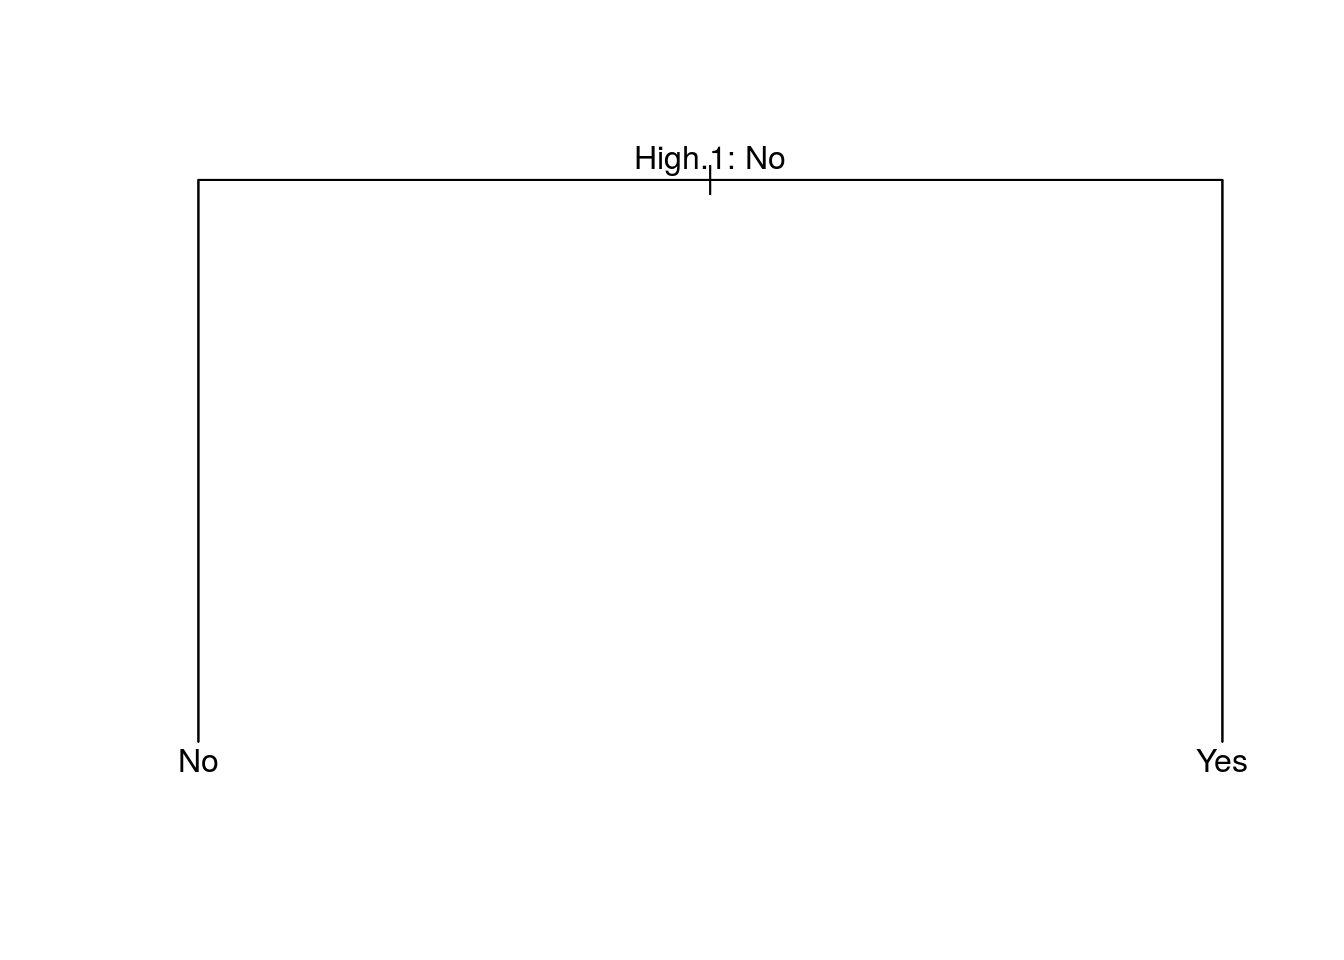
\includegraphics{GMwR_files/figure-latex/unnamed-chunk-1-1.pdf}

\begin{Shaded}
\begin{Highlighting}[]
\CommentTok{# igraph object}
\KeywordTok{library}\NormalTok{(igraph)}
\end{Highlighting}
\end{Shaded}

\begin{verbatim}
## 
## Attaching package: 'igraph'
\end{verbatim}

\begin{verbatim}
## The following objects are masked from 'package:graph':
## 
##     degree, edges, intersection, union
\end{verbatim}

\begin{verbatim}
## The following objects are masked from 'package:BiocGenerics':
## 
##     normalize, path, union
\end{verbatim}

\begin{verbatim}
## The following objects are masked from 'package:stats':
## 
##     decompose, spectrum
\end{verbatim}

\begin{verbatim}
## The following object is masked from 'package:base':
## 
##     union
\end{verbatim}

\begin{Shaded}
\begin{Highlighting}[]
\NormalTok{ug0i =}\StringTok{ }\KeywordTok{ug}\NormalTok{(}\OperatorTok{~}\NormalTok{a}\OperatorTok{:}\NormalTok{b}\OperatorTok{+}\NormalTok{b}\OperatorTok{:}\NormalTok{c}\OperatorTok{:}\NormalTok{d}\OperatorTok{+}\NormalTok{e, }\DataTypeTok{result =} \StringTok{"igraph"}\NormalTok{)}
\NormalTok{ug0i}
\end{Highlighting}
\end{Shaded}

\begin{verbatim}
## IGRAPH ef24c4c UNW- 5 4 -- 
## + attr: name (v/c), label (v/c), weight (e/n)
## + edges from ef24c4c (vertex names):
## [1] a--b b--c b--d c--d
\end{verbatim}

\begin{Shaded}
\begin{Highlighting}[]
\KeywordTok{plot}\NormalTok{(ug0i, }\DataTypeTok{layout =}\NormalTok{ layout.spring)}
\end{Highlighting}
\end{Shaded}

\begin{verbatim}
## Warning in v(graph): Spring layout was removed, we use Fruchterman-Reingold
## instead.
\end{verbatim}

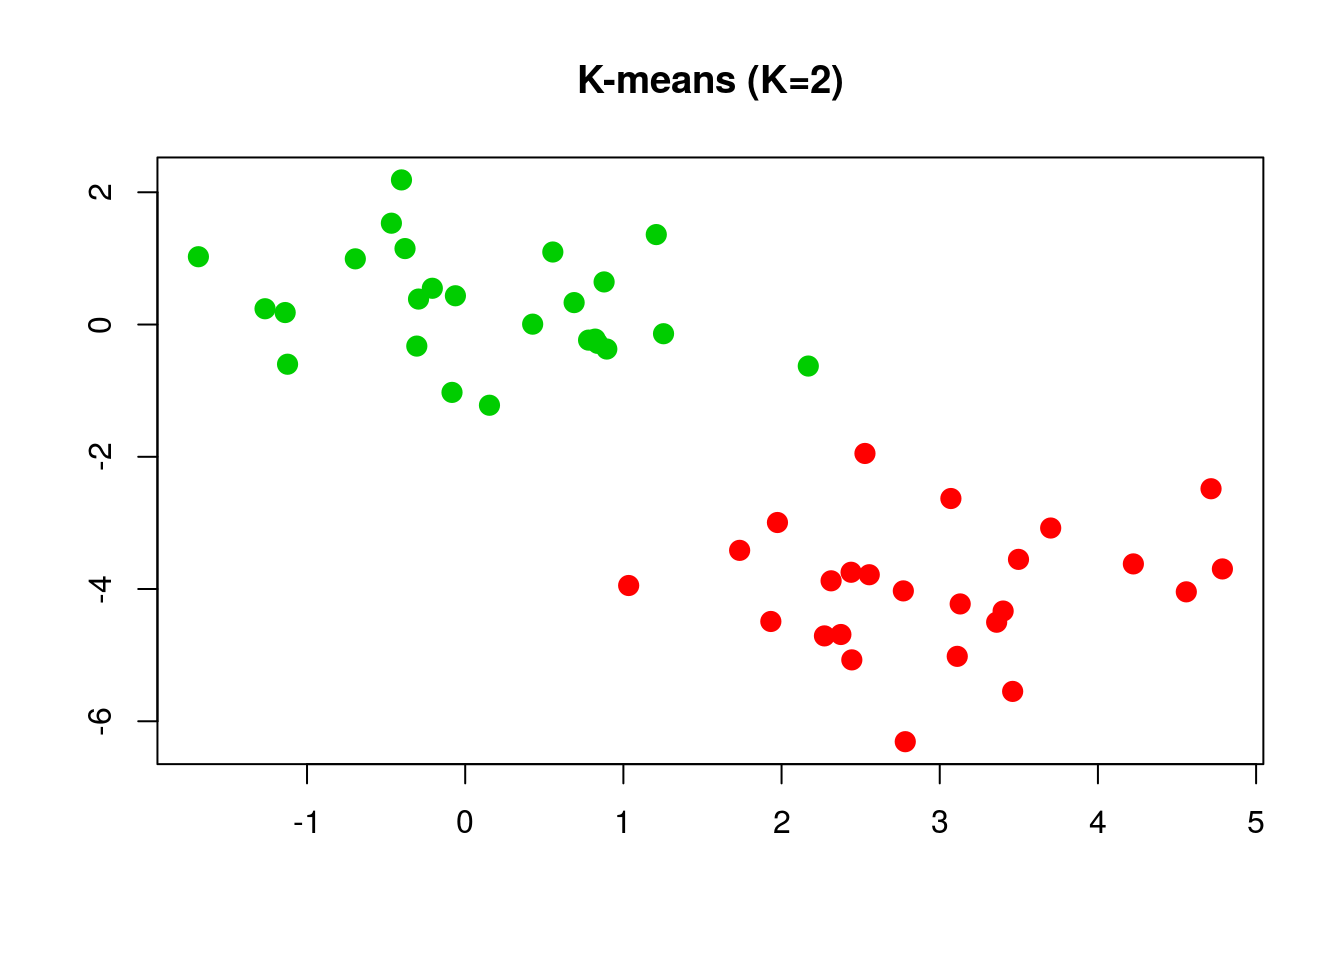
\includegraphics{GMwR_files/figure-latex/unnamed-chunk-2-1.pdf}

\begin{Shaded}
\begin{Highlighting}[]
\CommentTok{# customed plot function}
\NormalTok{myiplot =}\StringTok{ }\ControlFlowTok{function}\NormalTok{(x, ...)\{}
  \KeywordTok{V}\NormalTok{(x)}\OperatorTok{$}\NormalTok{size =}\StringTok{ }\DecValTok{30}
  \KeywordTok{V}\NormalTok{(x)}\OperatorTok{$}\NormalTok{label.cex =}\StringTok{ }\DecValTok{3}
  \KeywordTok{plot}\NormalTok{(x, ...)}
\NormalTok{\}}
\KeywordTok{myiplot}\NormalTok{(ug0i, }\DataTypeTok{layout =}\NormalTok{ layout.fruchterman.reingold)}
\end{Highlighting}
\end{Shaded}

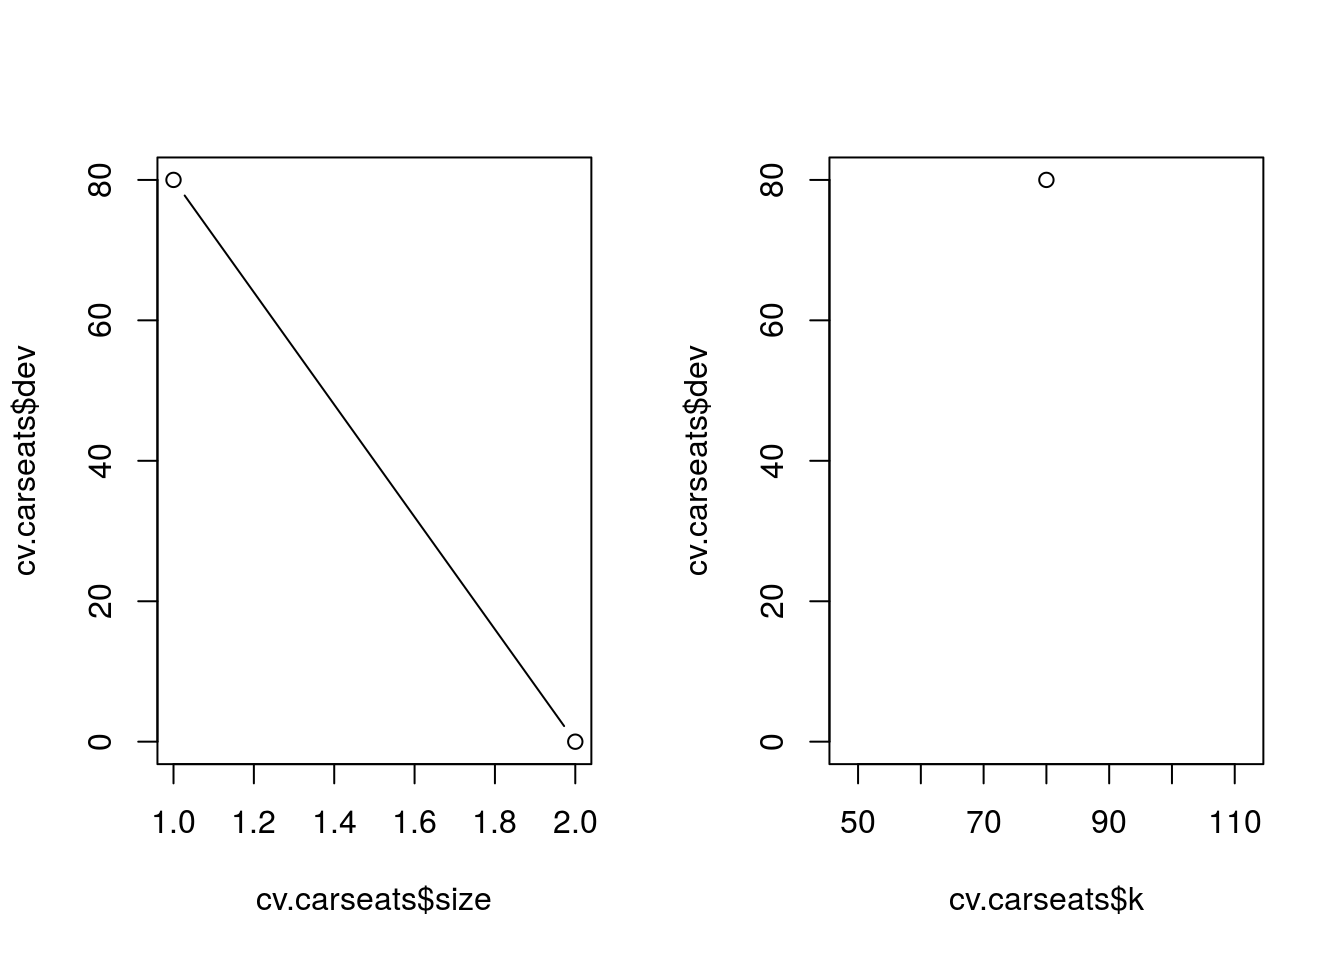
\includegraphics{GMwR_files/figure-latex/unnamed-chunk-3-1.pdf}

\begin{Shaded}
\begin{Highlighting}[]
\NormalTok{ug0a =}\StringTok{ }\KeywordTok{addEdge}\NormalTok{(}\StringTok{"a"}\NormalTok{, }\StringTok{"c"}\NormalTok{, ug0)}
\NormalTok{ug0a =}\StringTok{ }\KeywordTok{removeEdge}\NormalTok{(}\StringTok{"c"}\NormalTok{, }\StringTok{"d"}\NormalTok{, ug0)}
\KeywordTok{nodes}\NormalTok{(ug0)}
\end{Highlighting}
\end{Shaded}

\begin{verbatim}
## [1] "a" "b" "c" "d" "e"
\end{verbatim}

\begin{Shaded}
\begin{Highlighting}[]
\KeywordTok{edges}\NormalTok{(ug0)}
\end{Highlighting}
\end{Shaded}

\begin{verbatim}
## [[1]]
## A graphNEL graph with undirected edges
## Number of Nodes = 5 
## Number of Edges = 4 
## 
## attr(,"class")
## [1] "igraph.edge"
\end{verbatim}

\begin{Shaded}
\begin{Highlighting}[]
\KeywordTok{str}\NormalTok{(}\KeywordTok{edgeList}\NormalTok{(ug0))}
\end{Highlighting}
\end{Shaded}

\begin{verbatim}
## List of 4
##  $ : chr [1:2] "a" "b"
##  $ : chr [1:2] "b" "c"
##  $ : chr [1:2] "b" "d"
##  $ : chr [1:2] "c" "d"
\end{verbatim}

A clique is a maximal complete subset. The set of cliques of a graph
\(\cal G\) is denoted by \(\cal C(G)\).

NOTE: In literature the term clique is often used to denoted a complete
subset and may not necessarily be maximal.

\begin{Shaded}
\begin{Highlighting}[]
\KeywordTok{is.complete}\NormalTok{(ug0)}
\end{Highlighting}
\end{Shaded}

\begin{verbatim}
## [1] FALSE
\end{verbatim}

\begin{Shaded}
\begin{Highlighting}[]
\KeywordTok{is.complete}\NormalTok{(ug0, }\KeywordTok{c}\NormalTok{(}\StringTok{"b"}\NormalTok{, }\StringTok{"c"}\NormalTok{, }\StringTok{"d"}\NormalTok{))}
\end{Highlighting}
\end{Shaded}

\begin{verbatim}
## [1] TRUE
\end{verbatim}

\begin{Shaded}
\begin{Highlighting}[]
\KeywordTok{library}\NormalTok{(RBGL)}
\end{Highlighting}
\end{Shaded}

\begin{verbatim}
## 
## Attaching package: 'RBGL'
\end{verbatim}

\begin{verbatim}
## The following objects are masked from 'package:igraph':
## 
##     bfs, dfs, transitivity
\end{verbatim}

\begin{Shaded}
\begin{Highlighting}[]
\KeywordTok{maxClique}\NormalTok{(ug0)}
\end{Highlighting}
\end{Shaded}

\begin{verbatim}
## $maxCliques
## $maxCliques[[1]]
## [1] "b" "c" "d"
## 
## $maxCliques[[2]]
## [1] "b" "a"
## 
## $maxCliques[[3]]
## [1] "e"
\end{verbatim}

\begin{Shaded}
\begin{Highlighting}[]
\CommentTok{# or}
\KeywordTok{getCliques}\NormalTok{(ug0) }
\end{Highlighting}
\end{Shaded}

\begin{verbatim}
## [[1]]
## [1] "b" "c" "d"
## 
## [[2]]
## [1] "b" "a"
## 
## [[3]]
## [1] "e"
\end{verbatim}

path: \(\alpha = \alpha_0,\alpha_1,\ldots,\alpha_n=\beta\).

cycle: \(\alpha=\beta\).

separate: every path between a vertex in \(A\subset V\) and a vertex in
\(B\subset V\) contains a vertex from \(D\subset V\).

\begin{Shaded}
\begin{Highlighting}[]
\KeywordTok{separates}\NormalTok{(}\StringTok{"a"}\NormalTok{, }\StringTok{"d"}\NormalTok{, }\KeywordTok{c}\NormalTok{(}\StringTok{"b"}\NormalTok{, }\StringTok{"c"}\NormalTok{), ug0)}
\end{Highlighting}
\end{Shaded}

\begin{verbatim}
## [1] TRUE
\end{verbatim}

subgraph:

subgraph induced by \(A\subseteq V\):

\begin{Shaded}
\begin{Highlighting}[]
\NormalTok{ug1 =}\StringTok{ }\KeywordTok{subGraph}\NormalTok{(}\KeywordTok{c}\NormalTok{(}\StringTok{"b"}\NormalTok{, }\StringTok{"c"}\NormalTok{, }\StringTok{"d"}\NormalTok{, }\StringTok{"e"}\NormalTok{), ug0)}
\KeywordTok{plot}\NormalTok{(ug1)}
\end{Highlighting}
\end{Shaded}

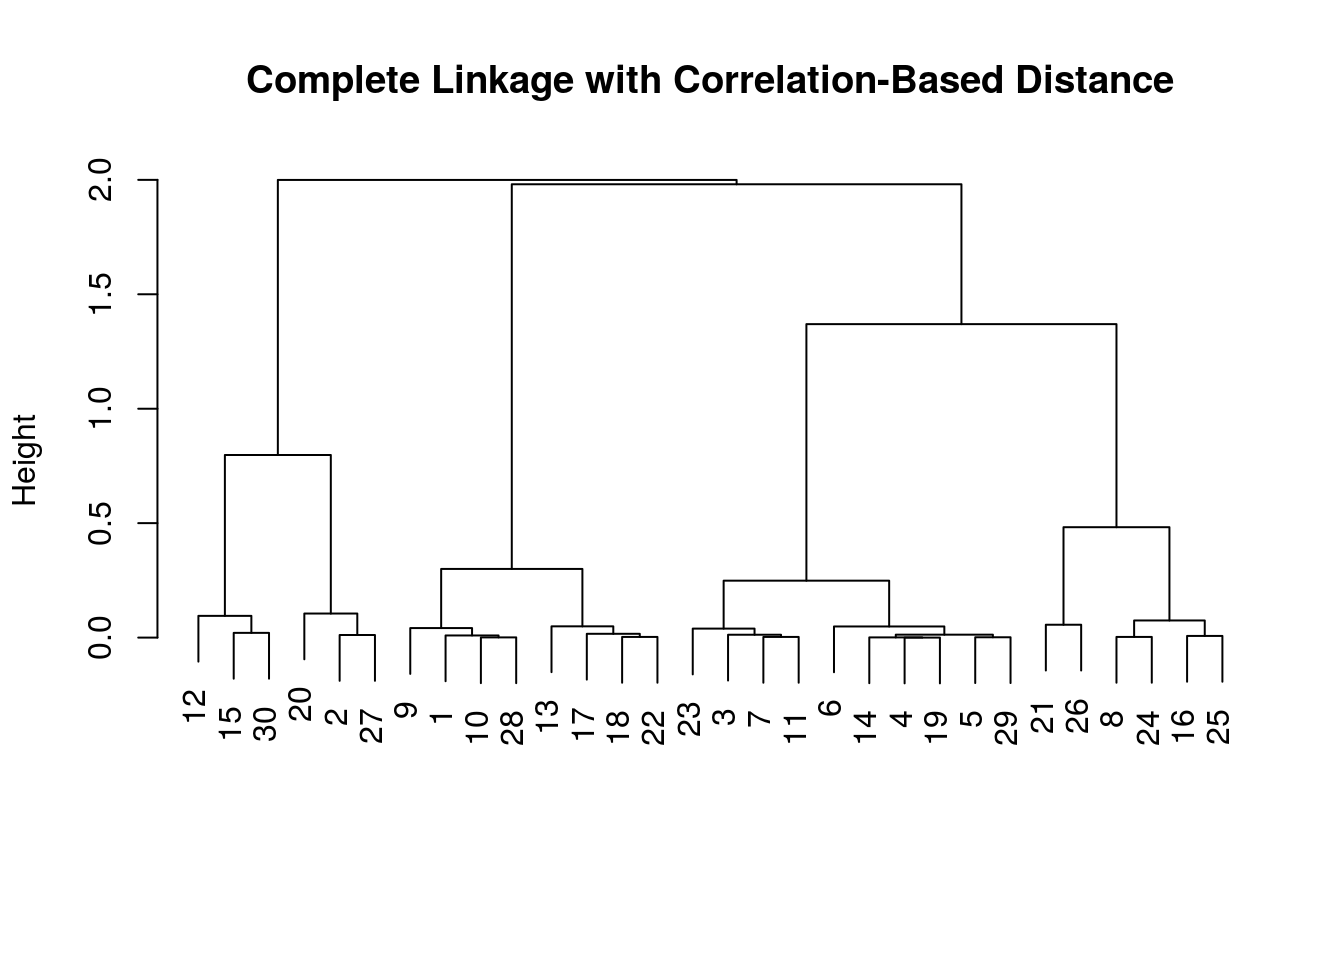
\includegraphics{GMwR_files/figure-latex/unnamed-chunk-7-1.pdf}

boundary: \(\mathrm{bd}(\alpha)=\mathrm{adj}(\alpha)\)

neighbours: \(\mathrm{ne}(\alpha)\)

closure: \(\mathrm{cl}(\alpha)=\mathrm{bd}(\alpha)\cup \{\alpha\}\).

\begin{Shaded}
\begin{Highlighting}[]
\KeywordTok{adj}\NormalTok{(ug0, }\StringTok{"c"}\NormalTok{)}
\end{Highlighting}
\end{Shaded}

\begin{verbatim}
## $c
## [1] "d" "b"
\end{verbatim}

\begin{Shaded}
\begin{Highlighting}[]
\KeywordTok{closure}\NormalTok{(}\StringTok{"c"}\NormalTok{, ug0)}
\end{Highlighting}
\end{Shaded}

\begin{verbatim}
## [1] "c" "d" "b"
\end{verbatim}

\subsection{Directed Acyclic Graphs}\label{directed-acyclic-graphs}

\begin{Shaded}
\begin{Highlighting}[]
\NormalTok{dag0 =}\StringTok{ }\KeywordTok{dag}\NormalTok{(}\OperatorTok{~}\NormalTok{a, }\OperatorTok{~}\NormalTok{b}\OperatorTok{*}\NormalTok{a, }\OperatorTok{~}\NormalTok{c}\OperatorTok{*}\NormalTok{a}\OperatorTok{*}\NormalTok{b, }\OperatorTok{~}\NormalTok{d}\OperatorTok{*}\NormalTok{c}\OperatorTok{*}\NormalTok{e, }\OperatorTok{~}\NormalTok{e}\OperatorTok{*}\NormalTok{a, }\OperatorTok{~}\NormalTok{g}\OperatorTok{*}\NormalTok{f)}
\NormalTok{dag0 =}\StringTok{ }\KeywordTok{dag}\NormalTok{(}\OperatorTok{~}\NormalTok{a}\OperatorTok{+}\NormalTok{b}\OperatorTok{*}\NormalTok{a}\OperatorTok{+}\NormalTok{c}\OperatorTok{*}\NormalTok{a}\OperatorTok{*}\NormalTok{b}\OperatorTok{+}\NormalTok{d}\OperatorTok{*}\NormalTok{c}\OperatorTok{*}\NormalTok{e}\OperatorTok{+}\NormalTok{e}\OperatorTok{*}\NormalTok{a}\OperatorTok{+}\NormalTok{g}\OperatorTok{*}\NormalTok{f)}
\NormalTok{dag0 =}\StringTok{ }\KeywordTok{dag}\NormalTok{(}\OperatorTok{~}\NormalTok{a}\OperatorTok{+}\NormalTok{b}\OperatorTok{|}\NormalTok{a}\OperatorTok{+}\NormalTok{c}\OperatorTok{|}\NormalTok{a}\OperatorTok{*}\NormalTok{b}\OperatorTok{+}\NormalTok{d}\OperatorTok{|}\NormalTok{c}\OperatorTok{*}\NormalTok{e}\OperatorTok{+}\NormalTok{e}\OperatorTok{|}\NormalTok{a}\OperatorTok{+}\NormalTok{g}\OperatorTok{|}\NormalTok{f)}
\NormalTok{dag0 =}\StringTok{ }\KeywordTok{dag}\NormalTok{(}\StringTok{"a"}\NormalTok{, }\KeywordTok{c}\NormalTok{(}\StringTok{"b"}\NormalTok{, }\StringTok{"a"}\NormalTok{), }\KeywordTok{c}\NormalTok{(}\StringTok{"c"}\NormalTok{, }\StringTok{"a"}\NormalTok{, }\StringTok{"b"}\NormalTok{), }\KeywordTok{c}\NormalTok{(}\StringTok{"d"}\NormalTok{, }\StringTok{"c"}\NormalTok{, }\StringTok{"e"}\NormalTok{), }\KeywordTok{c}\NormalTok{(}\StringTok{"e"}\NormalTok{, }\StringTok{"a"}\NormalTok{), }\KeywordTok{c}\NormalTok{(}\StringTok{"g"}\NormalTok{, }\StringTok{"f"}\NormalTok{))}
\NormalTok{dag0}
\end{Highlighting}
\end{Shaded}

\begin{verbatim}
## A graphNEL graph with directed edges
## Number of Nodes = 7 
## Number of Edges = 7
\end{verbatim}

\begin{Shaded}
\begin{Highlighting}[]
\KeywordTok{plot}\NormalTok{(dag0)}
\end{Highlighting}
\end{Shaded}

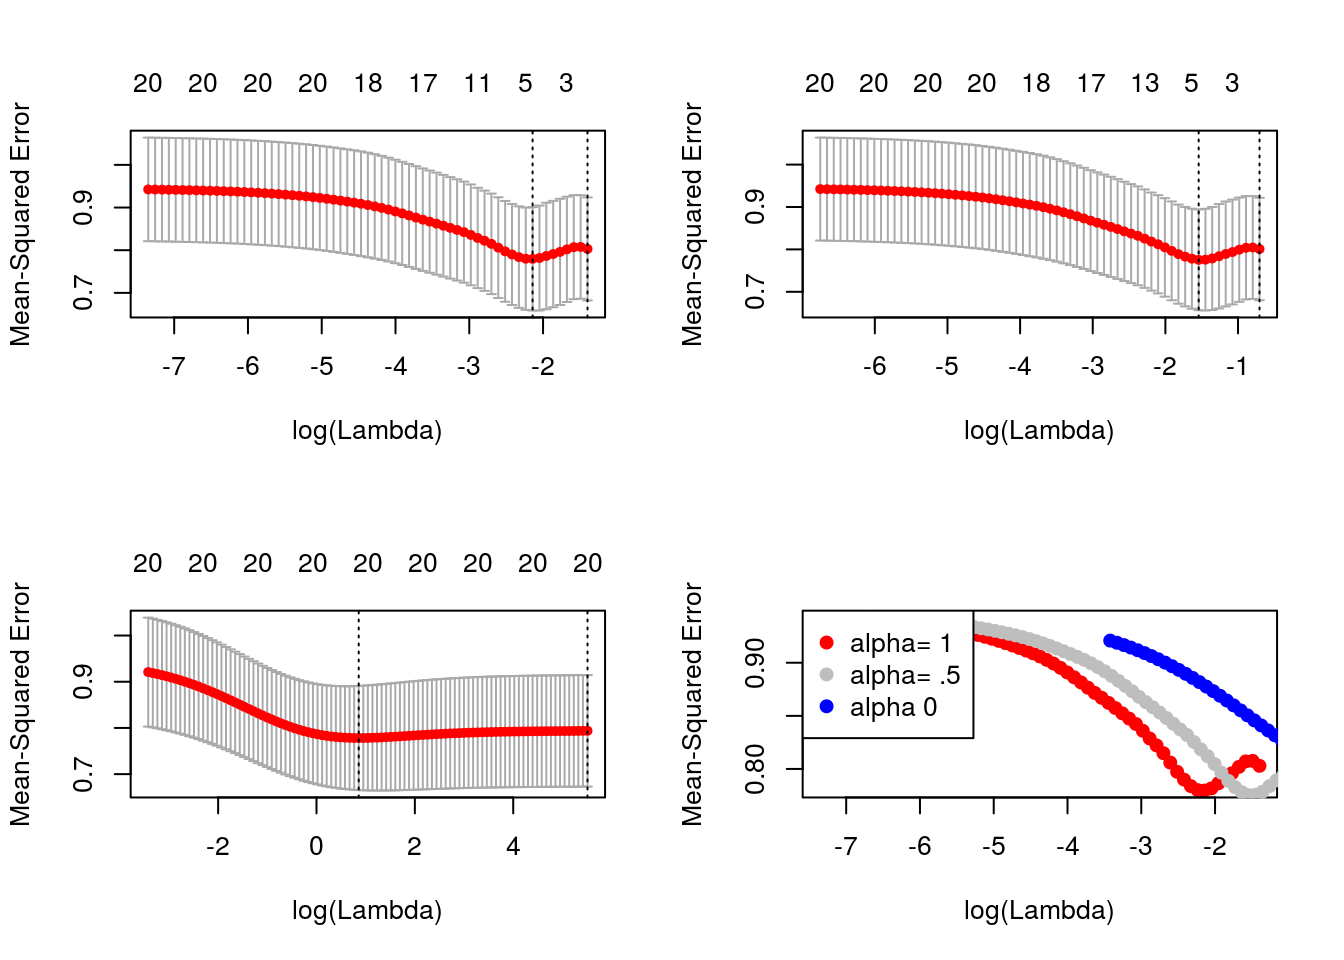
\includegraphics{GMwR_files/figure-latex/unnamed-chunk-9-1.pdf}

\begin{Shaded}
\begin{Highlighting}[]
\KeywordTok{nodes}\NormalTok{(dag0)}
\end{Highlighting}
\end{Shaded}

\begin{verbatim}
## [1] "a" "b" "c" "d" "e" "g" "f"
\end{verbatim}

\begin{Shaded}
\begin{Highlighting}[]
\KeywordTok{str}\NormalTok{(}\KeywordTok{edges}\NormalTok{(dag0))}
\end{Highlighting}
\end{Shaded}

\begin{verbatim}
## List of 1
##  $ :Formal class 'graphNEL' [package "graph"] with 6 slots
##   .. ..@ nodes     : chr [1:7] "a" "b" "c" "d" ...
##   .. ..@ edgeL     :List of 7
##   .. .. ..$ a:List of 1
##   .. .. .. ..$ edges: int [1:3] 2 3 5
##   .. .. ..$ b:List of 1
##   .. .. .. ..$ edges: int 3
##   .. .. ..$ c:List of 1
##   .. .. .. ..$ edges: int 4
##   .. .. ..$ d:List of 1
##   .. .. .. ..$ edges: num(0) 
##   .. .. ..$ e:List of 1
##   .. .. .. ..$ edges: int 4
##   .. .. ..$ g:List of 1
##   .. .. .. ..$ edges: num(0) 
##   .. .. ..$ f:List of 1
##   .. .. .. ..$ edges: int 6
##   .. ..@ edgeData  :Formal class 'attrData' [package "graph"] with 2 slots
##   .. .. .. ..@ data    :List of 7
##   .. .. .. .. ..$ a|b:List of 1
##   .. .. .. .. .. ..$ weight: num 1
##   .. .. .. .. ..$ a|c:List of 1
##   .. .. .. .. .. ..$ weight: num 1
##   .. .. .. .. ..$ a|e:List of 1
##   .. .. .. .. .. ..$ weight: num 1
##   .. .. .. .. ..$ b|c:List of 1
##   .. .. .. .. .. ..$ weight: num 1
##   .. .. .. .. ..$ c|d:List of 1
##   .. .. .. .. .. ..$ weight: num 1
##   .. .. .. .. ..$ e|d:List of 1
##   .. .. .. .. .. ..$ weight: num 1
##   .. .. .. .. ..$ f|g:List of 1
##   .. .. .. .. .. ..$ weight: num 1
##   .. .. .. ..@ defaults:List of 1
##   .. .. .. .. ..$ weight: num 1
##   .. ..@ nodeData  :Formal class 'attrData' [package "graph"] with 2 slots
##   .. .. .. ..@ data    : list()
##   .. .. .. ..@ defaults: list()
##   .. ..@ renderInfo:Formal class 'renderInfo' [package "graph"] with 4 slots
##   .. .. .. ..@ nodes: list()
##   .. .. .. ..@ edges: list()
##   .. .. .. ..@ graph: list()
##   .. .. .. ..@ pars : list()
##   .. ..@ graphData :List of 1
##   .. .. ..$ edgemode: chr "directed"
##  - attr(*, "class")= chr "igraph.edge"
\end{verbatim}

\begin{Shaded}
\begin{Highlighting}[]
\KeywordTok{str}\NormalTok{(}\KeywordTok{edgeList}\NormalTok{(dag0))}
\end{Highlighting}
\end{Shaded}

\begin{verbatim}
## List of 7
##  $ : chr [1:2] "a" "b"
##  $ : chr [1:2] "a" "c"
##  $ : chr [1:2] "a" "e"
##  $ : chr [1:2] "b" "c"
##  $ : chr [1:2] "c" "d"
##  $ : chr [1:2] "e" "d"
##  $ : chr [1:2] "f" "g"
\end{verbatim}

\begin{Shaded}
\begin{Highlighting}[]
\NormalTok{vpardag0 =}\StringTok{ }\KeywordTok{vpar}\NormalTok{(dag0)}
\NormalTok{vpardag0}\OperatorTok{$}\NormalTok{c}
\end{Highlighting}
\end{Shaded}

\begin{verbatim}
## [1] "c" "a" "b"
\end{verbatim}

path:

parents:

children:

ancestor:

ancestral set:

ancestral graph:

\begin{Shaded}
\begin{Highlighting}[]
\KeywordTok{parents}\NormalTok{(}\StringTok{"d"}\NormalTok{, dag0)}
\end{Highlighting}
\end{Shaded}

\begin{verbatim}
## [1] "c" "e"
\end{verbatim}

\begin{Shaded}
\begin{Highlighting}[]
\KeywordTok{children}\NormalTok{(}\StringTok{"c"}\NormalTok{, dag0)}
\end{Highlighting}
\end{Shaded}

\begin{verbatim}
## [1] "d"
\end{verbatim}

\begin{Shaded}
\begin{Highlighting}[]
\KeywordTok{ancestralSet}\NormalTok{(}\KeywordTok{c}\NormalTok{(}\StringTok{"b"}\NormalTok{, }\StringTok{"e"}\NormalTok{), dag0)}
\end{Highlighting}
\end{Shaded}

\begin{verbatim}
## [1] "a" "b" "e"
\end{verbatim}

\begin{Shaded}
\begin{Highlighting}[]
\KeywordTok{ancestralGraph}\NormalTok{(}\KeywordTok{c}\NormalTok{(}\StringTok{"b"}\NormalTok{, }\StringTok{"e"}\NormalTok{), dag0)}
\end{Highlighting}
\end{Shaded}

\begin{verbatim}
## A graphNEL graph with directed edges
## Number of Nodes = 3 
## Number of Edges = 2
\end{verbatim}

\begin{Shaded}
\begin{Highlighting}[]
\KeywordTok{plot}\NormalTok{(}\KeywordTok{ancestralGraph}\NormalTok{(}\KeywordTok{c}\NormalTok{(}\StringTok{"b"}\NormalTok{, }\StringTok{"e"}\NormalTok{), dag0))}
\end{Highlighting}
\end{Shaded}

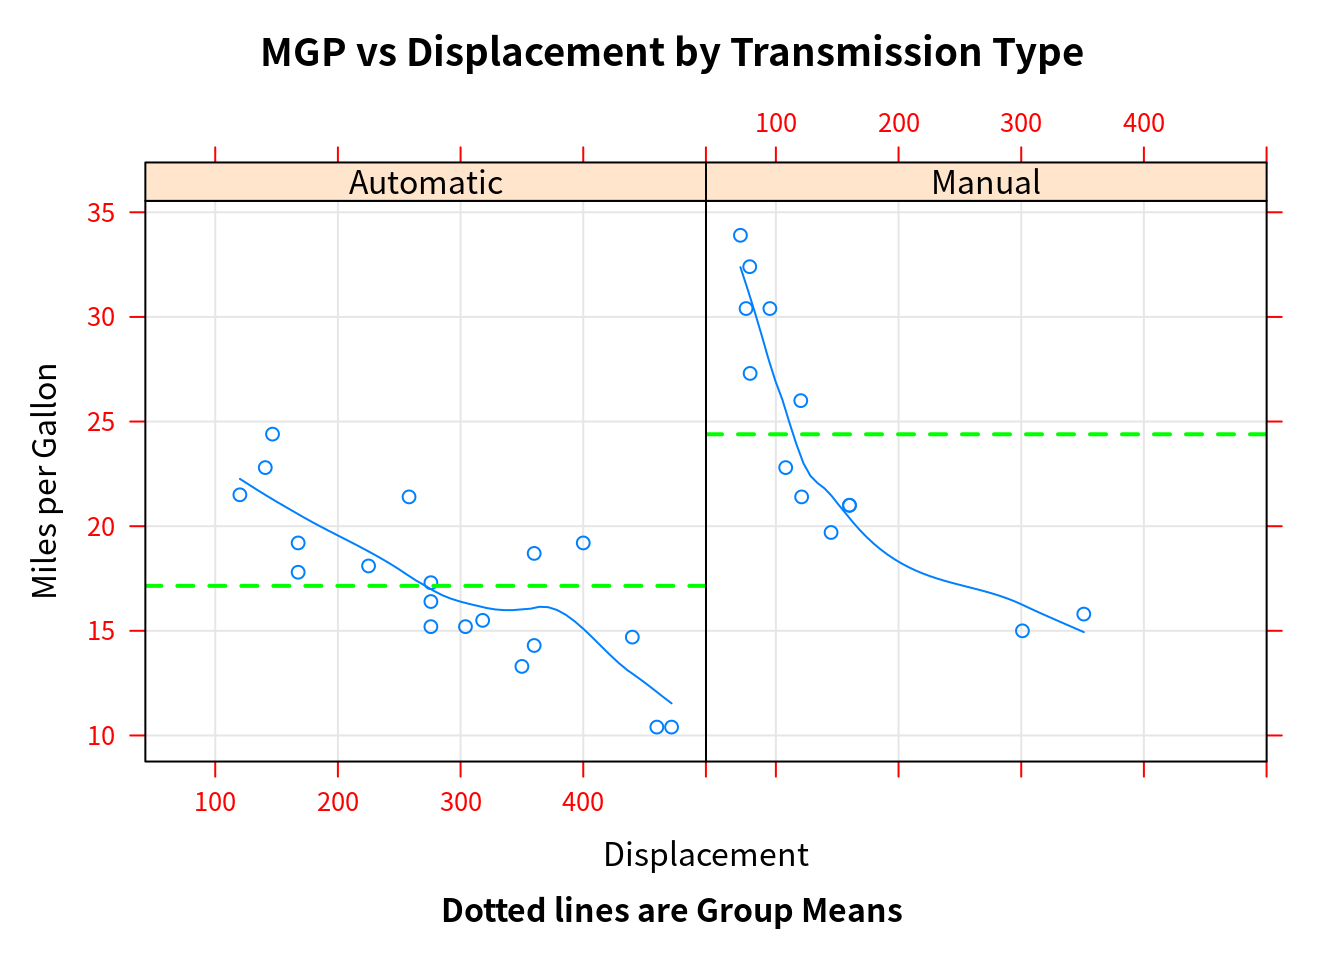
\includegraphics{GMwR_files/figure-latex/unnamed-chunk-11-1.pdf}

moralization:

\begin{enumerate}
\def\labelenumi{\arabic{enumi}.}
\tightlist
\item
  add edges between the parents of each node
\item
  replace all directed edges with undirected ones
\end{enumerate}

\begin{Shaded}
\begin{Highlighting}[]
\NormalTok{dag0m =}\StringTok{ }\KeywordTok{moralize}\NormalTok{(dag0)}
\KeywordTok{plot}\NormalTok{(dag0m)}
\end{Highlighting}
\end{Shaded}

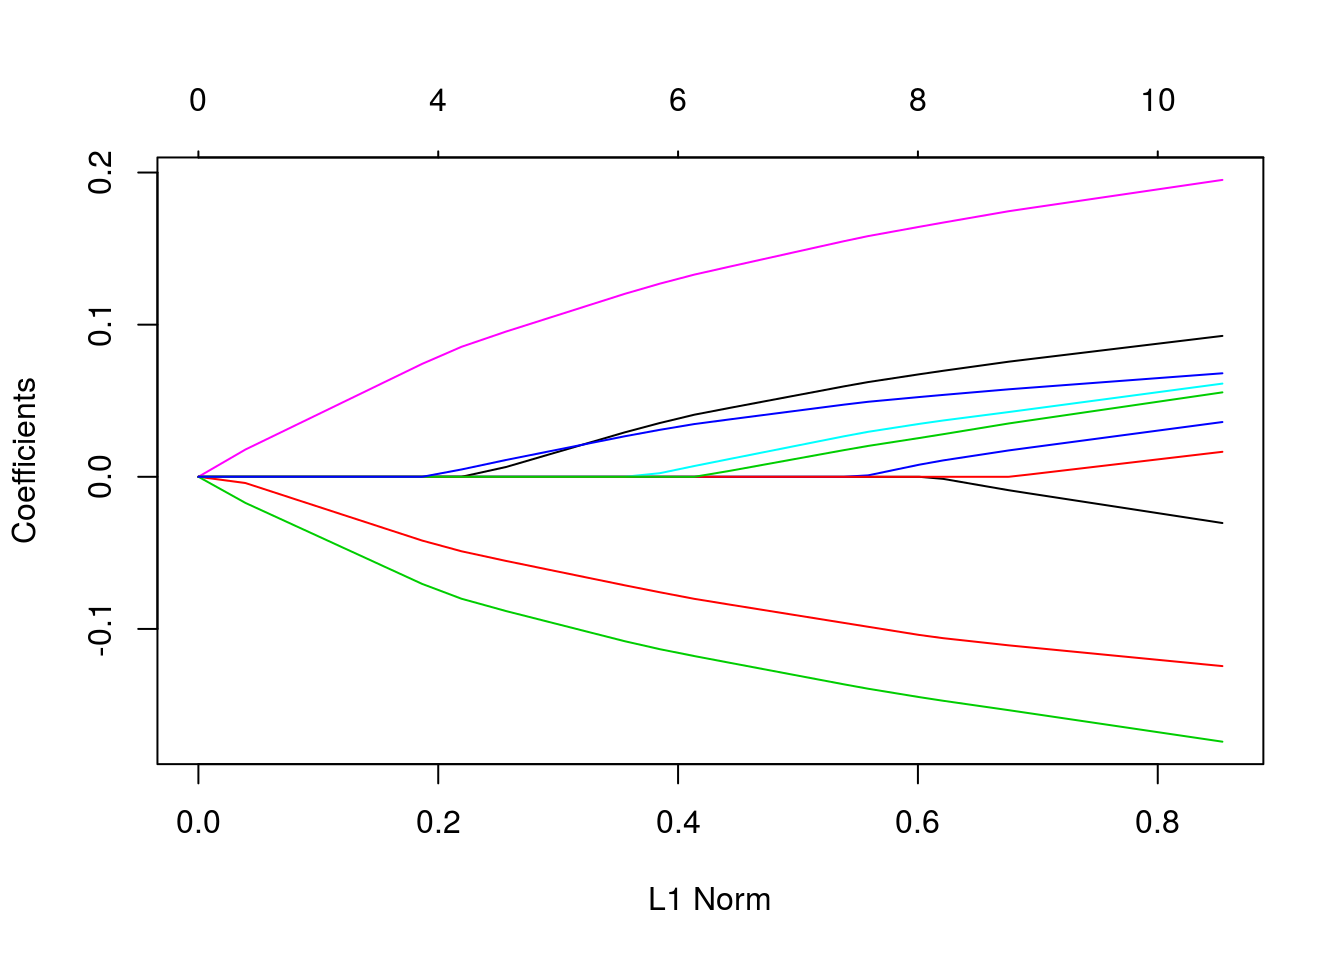
\includegraphics{GMwR_files/figure-latex/unnamed-chunk-12-1.pdf}

\subsection{Mixed Graphs}\label{mixed-graphs}

path: \(v_i-v_{i+1}\), \(v_i\leftrightarrow v_{i+1}\) or
\(v_i\rightarrow v_{i+1}\).

undirected: all are \(v_i-v_{i+1}\)

directed: all are \(v_i\rightarrow v_{i+1}\).

semi-directed (?): at least one \(v_i\rightarrow v_{i+1}\).

cycle: \(v_i=v_{k+1}\)

\begin{Shaded}
\begin{Highlighting}[]
\NormalTok{adjm =}\StringTok{ }\KeywordTok{matrix}\NormalTok{(}\KeywordTok{c}\NormalTok{(}\DecValTok{0}\NormalTok{,}\DecValTok{1}\NormalTok{,}\DecValTok{1}\NormalTok{,}\DecValTok{0}\NormalTok{,}\DecValTok{1}\NormalTok{,}\DecValTok{0}\NormalTok{,}\DecValTok{0}\NormalTok{,}\DecValTok{1}\NormalTok{,}\DecValTok{1}\NormalTok{,}\DecValTok{0}\NormalTok{,}\DecValTok{0}\NormalTok{,}\DecValTok{0}\NormalTok{,}\DecValTok{1}\NormalTok{,}\DecValTok{1}\NormalTok{,}\DecValTok{1}\NormalTok{,}\DecValTok{0}\NormalTok{), }\DataTypeTok{nrow=}\DecValTok{4}\NormalTok{)}
\KeywordTok{rownames}\NormalTok{(adjm) <-}\StringTok{ }\KeywordTok{colnames}\NormalTok{(adjm) <-}\StringTok{ }\NormalTok{letters[}\DecValTok{1}\OperatorTok{:}\DecValTok{4}\NormalTok{]}
\NormalTok{adjm}
\end{Highlighting}
\end{Shaded}

\begin{verbatim}
##   a b c d
## a 0 1 1 1
## b 1 0 0 1
## c 1 0 0 1
## d 0 1 0 0
\end{verbatim}

\begin{Shaded}
\begin{Highlighting}[]
\NormalTok{gG =}\StringTok{ }\KeywordTok{as}\NormalTok{(adjm, }\StringTok{"graphNEL"}\NormalTok{)}
\KeywordTok{plot}\NormalTok{(gG, }\StringTok{"neato"}\NormalTok{)}
\end{Highlighting}
\end{Shaded}

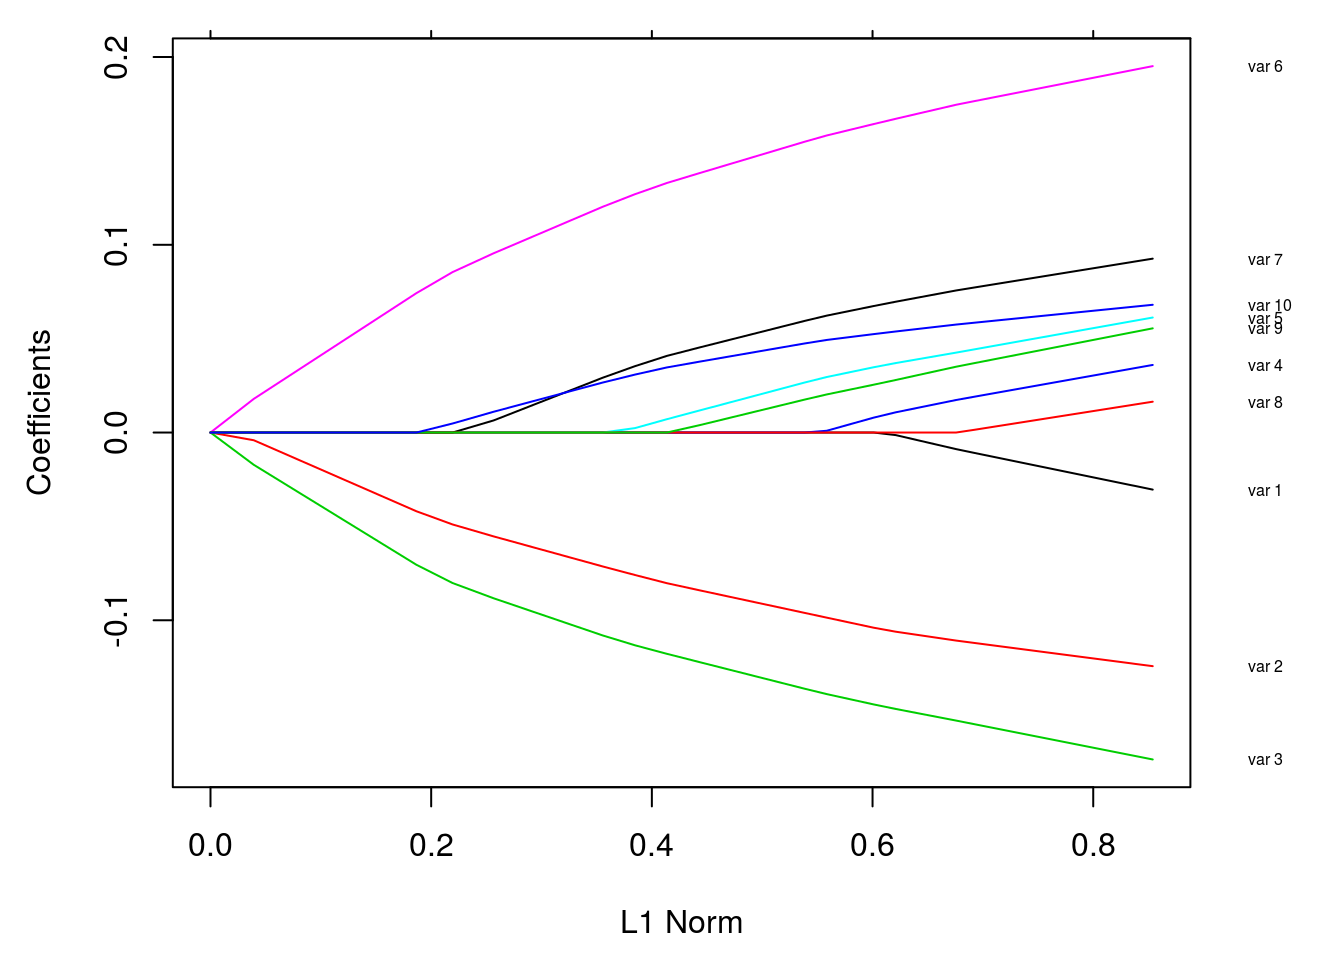
\includegraphics{GMwR_files/figure-latex/unnamed-chunk-13-1.pdf}

\begin{Shaded}
\begin{Highlighting}[]
\NormalTok{gG1 <-}\StringTok{ }\KeywordTok{as}\NormalTok{(adjm, }\StringTok{"igraph"}\NormalTok{)}
\KeywordTok{myiplot}\NormalTok{(gG1, }\DataTypeTok{layout =}\NormalTok{ layout.spring)}
\end{Highlighting}
\end{Shaded}

\begin{verbatim}
## Warning in v(graph): Spring layout was removed, we use Fruchterman-Reingold
## instead.
\end{verbatim}

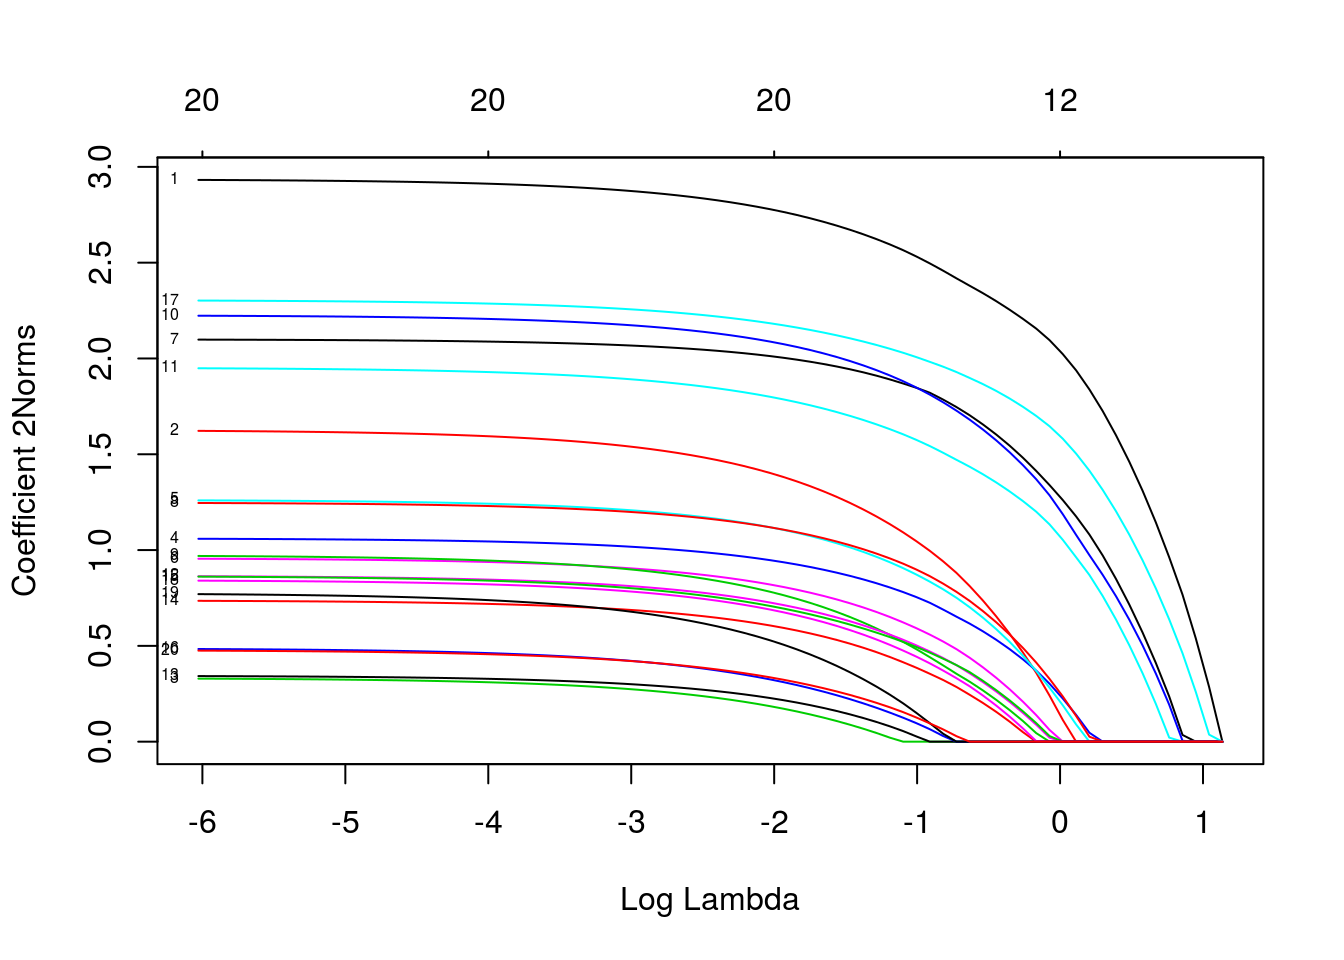
\includegraphics{GMwR_files/figure-latex/unnamed-chunk-14-1.pdf}

\begin{Shaded}
\begin{Highlighting}[]
\CommentTok{# display undirected instead of bidirected edges}
\KeywordTok{E}\NormalTok{(gG1)}\OperatorTok{$}\NormalTok{arrow.mode =}\StringTok{ }\KeywordTok{c}\NormalTok{(}\DecValTok{2}\NormalTok{, }\DecValTok{0}\NormalTok{)[}\DecValTok{1}\OperatorTok{+}\KeywordTok{is.mutual}\NormalTok{(gG1)]}
\KeywordTok{myiplot}\NormalTok{(gG1, }\DataTypeTok{layout =}\NormalTok{ layout.fruchterman.reingold)}
\end{Highlighting}
\end{Shaded}

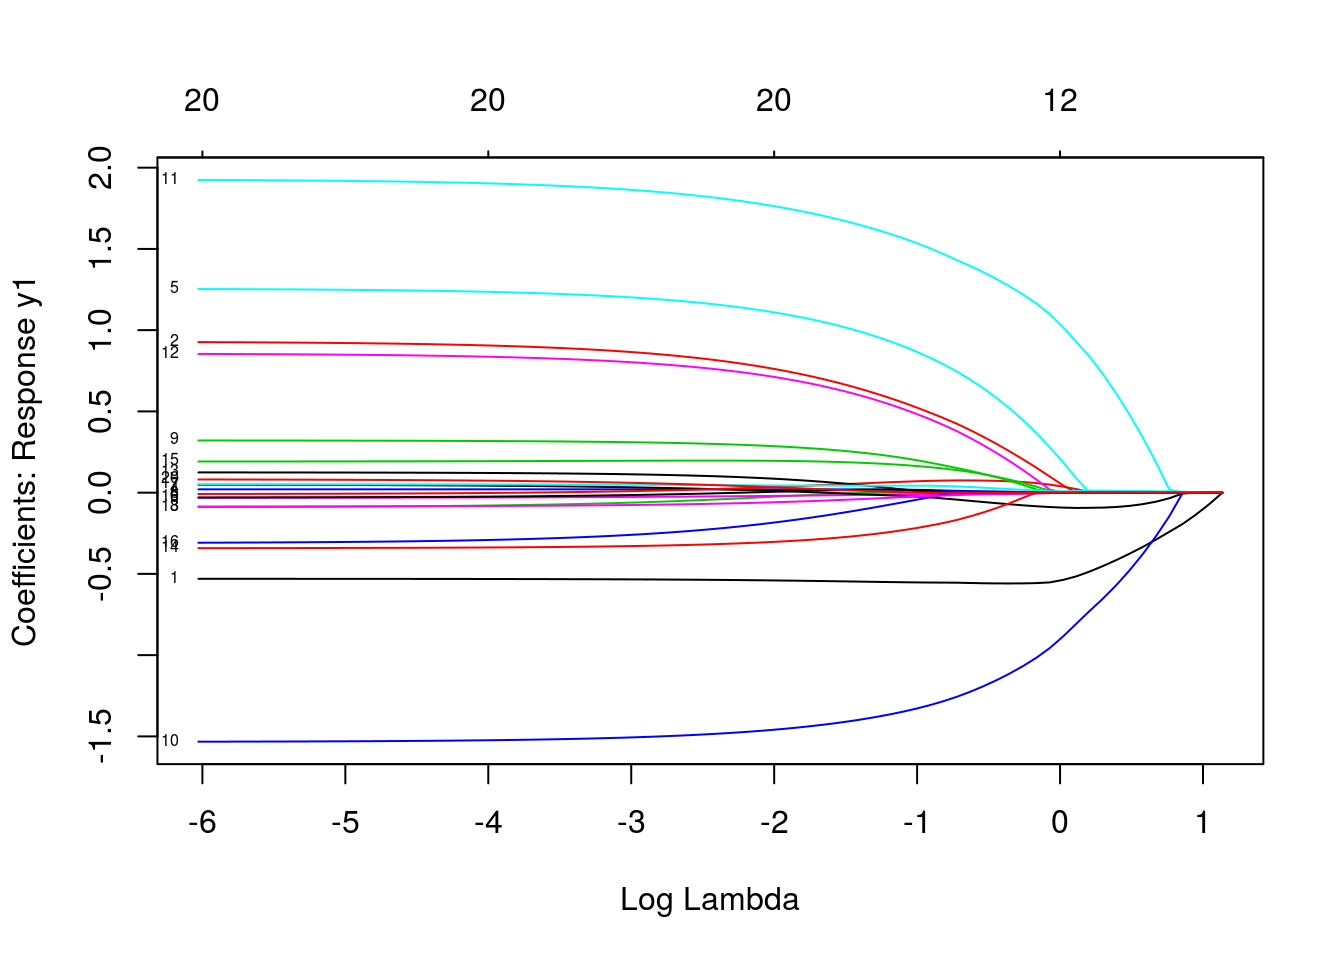
\includegraphics{GMwR_files/figure-latex/unnamed-chunk-14-2.pdf}

chain graph: mixed graph with no bidirected edges and no semi-directed
cycles

\begin{Shaded}
\begin{Highlighting}[]
\NormalTok{d1 =}\StringTok{ }\KeywordTok{matrix}\NormalTok{(}\DecValTok{0}\NormalTok{, }\DecValTok{11}\NormalTok{, }\DecValTok{11}\NormalTok{)}
\NormalTok{d1[}\DecValTok{1}\NormalTok{,}\DecValTok{2}\NormalTok{] <-}\StringTok{ }\NormalTok{d1[}\DecValTok{2}\NormalTok{,}\DecValTok{1}\NormalTok{] <-}\StringTok{ }\NormalTok{d1[}\DecValTok{1}\NormalTok{,}\DecValTok{3}\NormalTok{] <-}\StringTok{ }\NormalTok{d1[}\DecValTok{3}\NormalTok{,}\DecValTok{1}\NormalTok{] <-}\StringTok{ }\NormalTok{d1[}\DecValTok{2}\NormalTok{,}\DecValTok{4}\NormalTok{] <-}\StringTok{ }\NormalTok{d1[}\DecValTok{4}\NormalTok{,}\DecValTok{2}\NormalTok{] <-}\StringTok{ }\NormalTok{d1[}\DecValTok{5}\NormalTok{,}\DecValTok{6}\NormalTok{] <-}\StringTok{ }\NormalTok{d1[}\DecValTok{6}\NormalTok{,}\DecValTok{5}\NormalTok{] <-}\StringTok{ }\DecValTok{1}
\NormalTok{d1[}\DecValTok{9}\NormalTok{,}\DecValTok{10}\NormalTok{] <-}\StringTok{ }\NormalTok{d1[}\DecValTok{10}\NormalTok{,}\DecValTok{9}\NormalTok{] <-}\StringTok{ }\NormalTok{d1[}\DecValTok{7}\NormalTok{,}\DecValTok{8}\NormalTok{] <-}\StringTok{ }\NormalTok{d1[}\DecValTok{8}\NormalTok{,}\DecValTok{7}\NormalTok{] <-}\StringTok{ }\NormalTok{d1[}\DecValTok{3}\NormalTok{,}\DecValTok{5}\NormalTok{] <-}\StringTok{ }\NormalTok{d1[}\DecValTok{5}\NormalTok{,}\DecValTok{10}\NormalTok{] <-}\StringTok{ }\NormalTok{d1[}\DecValTok{4}\NormalTok{,}\DecValTok{6}\NormalTok{] <-}\StringTok{ }\NormalTok{d1[}\DecValTok{4}\NormalTok{,}\DecValTok{7}\NormalTok{] <-}\StringTok{ }\DecValTok{1}
\NormalTok{d1[}\DecValTok{6}\NormalTok{,}\DecValTok{11}\NormalTok{] <-}\StringTok{ }\NormalTok{d1[}\DecValTok{7}\NormalTok{,}\DecValTok{11}\NormalTok{] <-}\StringTok{ }\DecValTok{1}
\KeywordTok{rownames}\NormalTok{(d1) <-}\StringTok{ }\KeywordTok{colnames}\NormalTok{(d1) <-}\StringTok{ }\NormalTok{letters[}\DecValTok{1}\OperatorTok{:}\DecValTok{11}\NormalTok{]}
\NormalTok{cG1 <-}\StringTok{ }\KeywordTok{as}\NormalTok{(d1, }\StringTok{"igraph"}\NormalTok{)}
\KeywordTok{E}\NormalTok{(cG1)}\OperatorTok{$}\NormalTok{arrow.mode <-}\StringTok{ }\KeywordTok{c}\NormalTok{(}\DecValTok{2}\NormalTok{,}\DecValTok{0}\NormalTok{)[}\DecValTok{1}\OperatorTok{+}\KeywordTok{is.mutual}\NormalTok{(cG1)]}
\KeywordTok{myiplot}\NormalTok{(cG1, }\DataTypeTok{layout=}\NormalTok{layout.spring)}
\end{Highlighting}
\end{Shaded}

\begin{verbatim}
## Warning in v(graph): Spring layout was removed, we use Fruchterman-Reingold
## instead.
\end{verbatim}

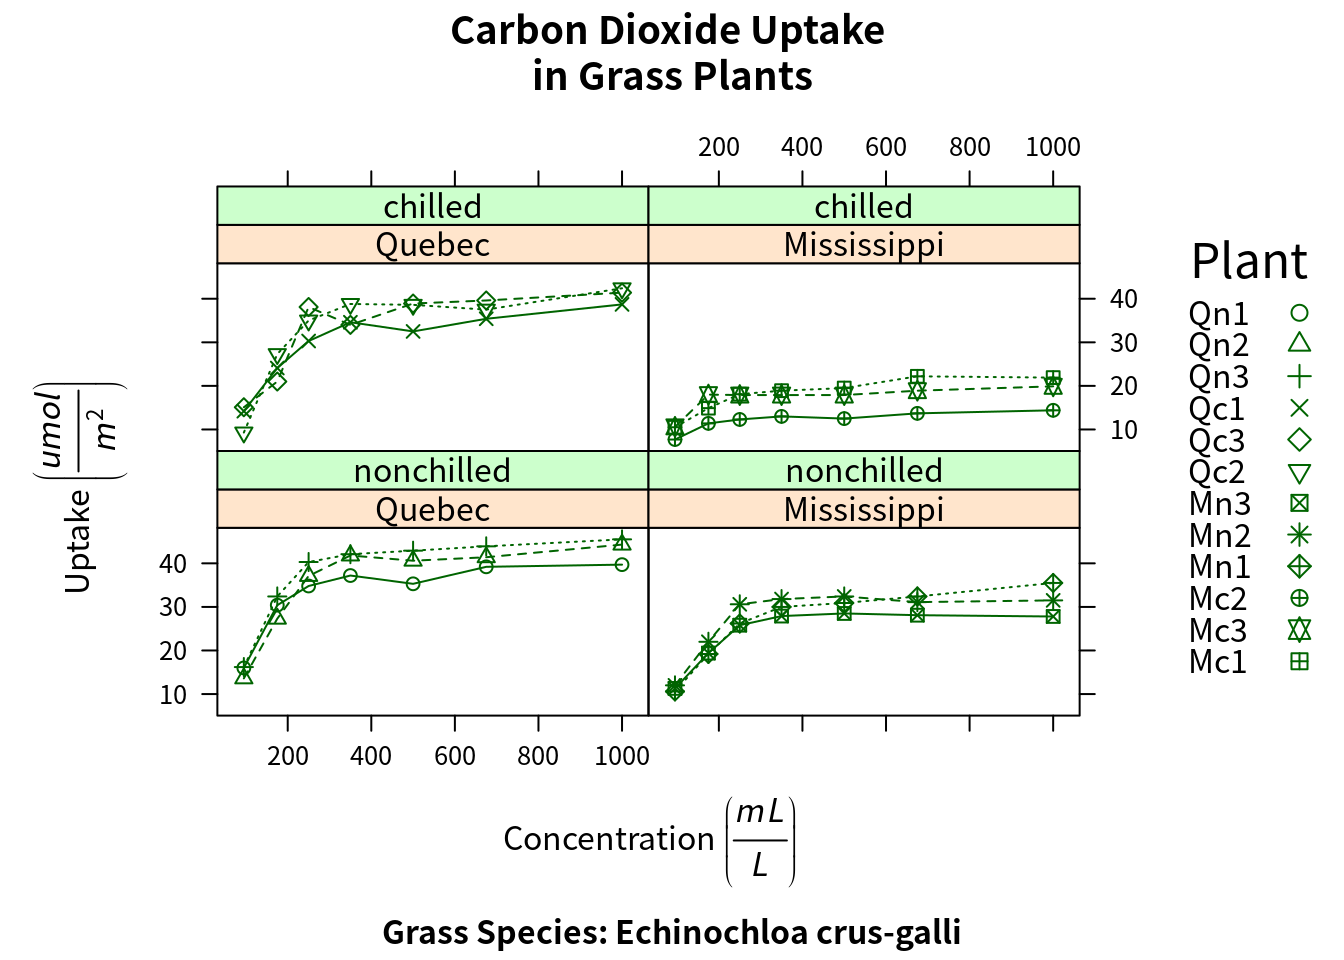
\includegraphics{GMwR_files/figure-latex/unnamed-chunk-15-1.pdf}

components: the connected components of the graph formed after removing
all directed edges from \(\cal G\). All edges within a component are
undirected, and all edges between components are directed. Also, all
arrows between any two components have the same direction.

\begin{Shaded}
\begin{Highlighting}[]
\CommentTok{# lcd package had been removed from CRAN}
\CommentTok{# the source package is also cannot be installed.}
\CommentTok{# so I extract the source code as follows (which depends on another package `ggm`)}
\KeywordTok{library}\NormalTok{(ggm)}
\end{Highlighting}
\end{Shaded}

\begin{verbatim}
## 
## Attaching package: 'ggm'
\end{verbatim}

\begin{verbatim}
## The following object is masked from 'package:igraph':
## 
##     pa
\end{verbatim}

\begin{Shaded}
\begin{Highlighting}[]
\StringTok{`}\DataTypeTok{is.chaingraph}\StringTok{`}\NormalTok{ <-}
\ControlFlowTok{function}\NormalTok{(amat)}
\NormalTok{\{}
\NormalTok{    wmat <-}\StringTok{ }\KeywordTok{matrix}\NormalTok{(}\KeywordTok{as.integer}\NormalTok{((amat }\OperatorTok{+}\StringTok{ }\KeywordTok{t}\NormalTok{(amat)) }\OperatorTok{>}\StringTok{ }\DecValTok{1}\NormalTok{), }\DataTypeTok{nrow =} \KeywordTok{nrow}\NormalTok{(amat))}
\NormalTok{    wg <-}\StringTok{ }\KeywordTok{graph.adjacency}\NormalTok{(wmat, }\DataTypeTok{mode =} \StringTok{"undirected"}\NormalTok{)}
\NormalTok{    cc <-}\StringTok{ }\KeywordTok{clusters}\NormalTok{(wg)}
\NormalTok{    neworder <-}\StringTok{ }\KeywordTok{order}\NormalTok{(cc}\OperatorTok{$}\NormalTok{membership)}
\NormalTok{    a <-}\StringTok{ }\KeywordTok{matrix}\NormalTok{(}\DecValTok{0}\NormalTok{, }\DataTypeTok{nrow =} \KeywordTok{length}\NormalTok{(cc}\OperatorTok{$}\NormalTok{csize), }\DataTypeTok{ncol =} \KeywordTok{length}\NormalTok{(cc}\OperatorTok{$}\NormalTok{csize))}
\NormalTok{    b <-}\StringTok{ }\KeywordTok{cumsum}\NormalTok{(cc}\OperatorTok{$}\NormalTok{csize)}
\NormalTok{    wmat <-}\StringTok{ }\NormalTok{amat[neworder, neworder]}
    \ControlFlowTok{for}\NormalTok{(i }\ControlFlowTok{in} \DecValTok{1}\OperatorTok{:}\StringTok{ }\KeywordTok{length}\NormalTok{(cc}\OperatorTok{$}\NormalTok{csize))\{}
        \ControlFlowTok{for}\NormalTok{(j }\ControlFlowTok{in} \DecValTok{1}\OperatorTok{:}\StringTok{ }\KeywordTok{length}\NormalTok{(cc}\OperatorTok{$}\NormalTok{csize))\{}
            \ControlFlowTok{if}\NormalTok{(j }\OperatorTok{!=}\StringTok{ }\NormalTok{i)\{}
\NormalTok{                a[i,j] <-}\StringTok{ }\KeywordTok{as.integer}\NormalTok{(}\KeywordTok{sum}\NormalTok{(wmat[(}\KeywordTok{max}\NormalTok{(b[i}\OperatorTok{-}\DecValTok{1}\NormalTok{],}\DecValTok{0}\NormalTok{)}\OperatorTok{+}\DecValTok{1}\NormalTok{)}\OperatorTok{:}\NormalTok{b[i],}
\NormalTok{                                              (}\KeywordTok{max}\NormalTok{(b[j}\OperatorTok{-}\DecValTok{1}\NormalTok{],}\DecValTok{0}\NormalTok{)}\OperatorTok{+}\DecValTok{1}\NormalTok{)}\OperatorTok{:}\NormalTok{b[j]]) }\OperatorTok{>}\StringTok{ }\DecValTok{0}\NormalTok{)}
\NormalTok{            \}}
\NormalTok{        \}}
\NormalTok{    \}}
    \KeywordTok{rownames}\NormalTok{(a) <-}\StringTok{ }\KeywordTok{colnames}\NormalTok{(a) <-}\StringTok{ }\KeywordTok{as.character}\NormalTok{(}\DecValTok{1}\OperatorTok{:}\KeywordTok{length}\NormalTok{(b))}
\NormalTok{    output <-}\StringTok{ }\KeywordTok{isAcyclic}\NormalTok{(a)}
    \ControlFlowTok{for}\NormalTok{(i }\ControlFlowTok{in} \DecValTok{1}\OperatorTok{:}\KeywordTok{length}\NormalTok{(b))\{}
\NormalTok{        temp <-}\StringTok{ }\NormalTok{wmat[(}\KeywordTok{max}\NormalTok{(b[i}\OperatorTok{-}\DecValTok{1}\NormalTok{],}\DecValTok{0}\NormalTok{)}\OperatorTok{+}\DecValTok{1}\NormalTok{)}\OperatorTok{:}\NormalTok{b[i], (}\KeywordTok{max}\NormalTok{(b[i}\OperatorTok{-}\DecValTok{1}\NormalTok{],}\DecValTok{0}\NormalTok{)}\OperatorTok{+}\DecValTok{1}\NormalTok{)}\OperatorTok{:}\NormalTok{b[i]]}
        \ControlFlowTok{if}\NormalTok{ (}\OperatorTok{!}\KeywordTok{all}\NormalTok{(temp }\OperatorTok{==}\StringTok{ }\KeywordTok{t}\NormalTok{(temp))) \{}
\NormalTok{            output <-}\StringTok{ }\OtherTok{FALSE}
            \ControlFlowTok{break}
\NormalTok{        \}}
\NormalTok{    \}}
\NormalTok{    chainorder <-}\StringTok{ }\KeywordTok{topOrder}\NormalTok{(a)}
\NormalTok{    vertorder<-}\KeywordTok{c}\NormalTok{()}
\NormalTok{    chainsize<-}\KeywordTok{c}\NormalTok{()}
    \ControlFlowTok{if}\NormalTok{(output }\OperatorTok{==}\StringTok{ }\OtherTok{TRUE}\NormalTok{)\{}
        \ControlFlowTok{for}\NormalTok{(k }\ControlFlowTok{in} \DecValTok{1}\OperatorTok{:}\KeywordTok{length}\NormalTok{(b))\{}
\NormalTok{            ## vertorder <- c(vertorder, which(cc$membership == chainorder[k]-1))}
\NormalTok{            vertorder <-}\StringTok{ }\KeywordTok{c}\NormalTok{(vertorder, }\KeywordTok{which}\NormalTok{(cc}\OperatorTok{$}\NormalTok{membership }\OperatorTok{==}\StringTok{ }\NormalTok{chainorder[k]))}
\NormalTok{            chainsize <-}\StringTok{ }\KeywordTok{c}\NormalTok{(chainsize, cc}\OperatorTok{$}\NormalTok{csize[chainorder[k]])}
\NormalTok{        \}}
\NormalTok{    \}}
    \KeywordTok{return}\NormalTok{(}\KeywordTok{list}\NormalTok{(}\DataTypeTok{result =}\NormalTok{ output,}
                \DataTypeTok{vert.order =}\NormalTok{ vertorder,}
                \DataTypeTok{chain.size =}\NormalTok{ chainsize))}
\NormalTok{\}}
\KeywordTok{is.chaingraph}\NormalTok{(}\KeywordTok{as}\NormalTok{(cG1, }\StringTok{"matrix"}\NormalTok{))}
\end{Highlighting}
\end{Shaded}

\begin{verbatim}
## $result
## [1] TRUE
## 
## $vert.order
##  [1]  1  2  3  4  5  6  7  8  9 10 11
## 
## $chain.size
## [1] 4 2 2 2 1
\end{verbatim}

condition independence graph (CIG): or Markov graph

One way to construct the CIG: first draw the complete graph, and then
remove those conditional independent pairs.

In \(k\) dimensions, there are \(2^{\binom{k}{2}}\) different graphs. If
it also includes the subgraph, the number of figures would be

\[
\sum_{i=0}^k\binom{k}{i}2^{\binom{i}{2}}
\]

\begin{theorem}
The separation theorem
\end{theorem}


\end{document}
